\begin{chapter}{Decision Support for Offshore Wind \label{Ch:ds-for-ow}}
Consider the problem of storing spare parts for an offshore wind farm which can be used to repair subassemblies. These spare parts will be used when subassemblies suffer a `serious' failure. Spare parts may be stored in a warehouse near to the dock at which spare parts will be loaded onto a boat so the spare can be shipped out to the turbine to be repaired. This is a question others have addressed. \citet{Tracht2013} perform a scenario analysis which investigates the limited availablity of spare compoents and equipment on preventative maintenance. A review of various models used for analysing spare parts strategies are given in \citet{Tusar2022}. The review stresses that not enough work is being done on constructing an optimal combination of spare parts, which is something we aim to address. The review suggests most analysts are interesting in minimising downtime; we will consider downtime (downtime is essentially the opposite of availablity) as well as other attributes to the problem. We also aim to incorporate sources of uncertainty into our analysis which is typically not done. A key difference with our approach will be that we use ideas from the history matching and BayesOpt literature to construct a set of sensible decisions that can be made. That is, we do not suppose that there is one `true' best strategy.

\section{The decision problem}

The Athena simulator models a turbine as being composed of $8$ important sub-assemblies and a ninth `catch all' subassembly. The DM has two problems to solve simultaneously:
\begin{itemize}
  \item[1.] Which warehouse, from a set of candidate warehouses, should the spare parts be stored in?
  \item[2.] What is the best way to manage the warehouse?
\end{itemize}
Good management of a suboptimal warehouse choice may be much better than bad management of the optimal warehouse choice. Of course, we would strive for good management of the optimal choice of warehouse. The managenent of the warehouse is described as follows:
\begin{itemize}
  \item[1.] How many spare parts should we store for each subassembly?
  \item[2.] At what point should we buy in more spare parts for the subassembly?
\end{itemize}
Almost every problem so far in this thesis has been adressed with decision theory. That theme is not going to end on page \thepage. We therefore need to formulate a utility function over all relevant attributes and specify an appropriate prior distribution over uncertain quantities. This example, although involved, will be illustrative. We do not directly specify any particular prior distribution; much work has been done on eliciting parameters for Athena by previous authours thus we adopt their priors. We will act as the decision maker, and analyst, in this excercise thus will specify the utility function on our own. The utility function will express sensible preferences, but they do not represent the preferences of real person.
\section{Mathematical formulation of the decision problem}
Here we will formuluate the decision problem following the guidelines illustrated by \citet{Smith2010}. Our problem is to choose a warehouse, $w_k$, of size $W_k$, and fill the warehouse with spare parts for each of the $9$ subassemblies.  We will allocate $s_i$ spares for subassembly $i$. We also need to construct a policy for restoring the numbers of spare parts as they deplete to ensure smooth running of the warehouse.

 We begin by formulating an appropriate set of attributes and we then specify our preferences though several marginal utility functions which will be combined into a single multi-attribute utility function. The first stage of elicitation of a utility function is to define all attributes relevant to the problem.

\subsubsection{Relevant attributes}

There are many attributes relevant to this problem. The key attributes to the problem are:
\begin{itemize}
  \item The availability time series (performance) of the wind farm
  \item The choice and cost of the warehouse in which spare parts are stored
  \item The number of spares of each type of subassembly
  \item The policy which dictates when to buy in more spare parts.
\end{itemize}
There may be many more attributes a decision maker would consider, but this is enough in our case to demonstrate the complexity of the problem and the application of appropriate methodology. We would next need to decide what the consequences, $c_i$, of any possible decision would be. The consequences of any decision are given in \cref{Tab:consequences} alongside information about the consequences. For example, the availability time series output by Athena over a $5$ years period, is internally processed by Athena and a length $240$ vector is output. We know that this time series is stochastic. The cost of the warehouse could be argued to be stochastic (for example, if the unit is rented, the owner may increase the rent to some uncertain value at some uncertain future time point). We however assume that the cost is fixed and later model this cost in terms of size. In \cref{Tab:consequences} we introduce the notation $\mathcal{S}^k_n$. This is the $k$ dimesional discrete simplex which we will define as
\begin{equation}
  \mathcal{S}^k_n = \left\{\bx \mid \sum_{i=1}^{k+1} = n, x_i \geq 1, x_i \in \{1, 2, \ldots, n-k+1\} \right\}.
\end{equation}
We have chosen to define $\mathcal{S}^k_n$ in this way as it reflects aspects of our application. A warehouse of size $n$ can have a minimum of $1$ spare part of type $i$ and can have at most $n-k+1$ spare parts of type $i$. This is because the other $k-1$ types of component all need at least $1$ spare part.
%decisions
\begin{table}[H]
	\centering
	\begin{tabular}{llrl}
		\toprule
    Label & Description & Parameter Space & Stochastic?\\\cmidrule{1-4}
    $c_1$ & Availability time series & $c_1 \in (0, 1)^{240}$& Yes\\
    $c_2$ & Choice of the restoration policy &$c_2 \in  (1, 99)^9$&  No\\
    $c_3$ &  Warehouse size & $c_3 \in \{50,  75, 100\}$& No\\\bottomrule
	\end{tabular}
	\caption{Summary of the consequences of a future decision to be made. These variables cause changes in the stochastic and deterministic consequences and it is the decisions themselves that will form the inputs of a future emulator.	The stochastic column describes how we model the consequence. \label{Tab:consequences}}
\end{table}
%consequences
\begin{table}[H]
	\centering
	\begin{tabular}{llr}
		\toprule
    Label & Description & Parameter Space\\\cmidrule{1-3}
    $x_1$--$x_9$ & Number of spare parts & $x_{1:9} \in \mathcal{S}^{8}_{x_{19}}$\\
    $x_{10}$--$x_{18}$ & Critical Percentages & $x_i \in (1,99)$\\
    $x_{19}$ & Warehouse size  (number of parts) & $\{ 50, 75, 100 \}$\\\bottomrule
	\end{tabular}
	\caption{Summary of the attributes of the decision problem. These are the variables for which individual utility functions will be elicted to be combined into an overall utility function.	\label{Tab:consequences}}
\end{table}
Our approach to eliciting the utility function will follow the advice of \citet{Smith2010} and \citet{Keeney1976}.  We assume that consequences are mutuallty utility independent, elicit a marginal utility function for each consequence using probability or certainty equivalents and then combine the marginal utility functions into an overall utility function via a multiplicative or additive form, depending on the preferences of the decision maker.
\section{The marginal utility functions}
Utility functions are unique upto positive affine transformations. That is, $au(x) + b$ expresses exactly the same preferences as $u(x)$ for any $a > 0$ and $b \in \R$. For this reason, we will construct all utilility functions on the unit interval. This also allows for easier elicitation as utilility and probability will be on the same scale. Likewise, all consequences will be on the unit interval.
\subsubsection{Utility of Availability}
The availability is a time series. At time $t$, denote the (random) availability by $A(t)$. The utility of some time series may be time dependent, however, in this problem we will work with the assumption that a fixed availability has constant utility, with respect to time. That is, $u(A(t), t)  = u(A(t))$ which is independent of $t$. We would then take the utility of the entire time series to be
\begin{equation}
  u_1(c_1)  = \frac{1}{240}\sum_{j = 1}^{240} \tilde{u}_{1}(c_1(t_j))
\end{equation}
where $\tilde{u}_{1}$ is the utility function for the availability at time $t$. This is just point-wise utility averaged over time. This average could be weighted if high availability is more important at some time points than others.

For the utility at time $t$, we believe a sigmoidal utility function would be appropriate. The reason being that, for regions of high availability, we would be risk-averse in trying to increase availability. However, whenever the availability is very low, we would be risk-seeking in order to ensure a profit it made. A sigmoidal utility function also has other useful reflections of our beliefs, for example, all very low availabilities are bad; an availablity of $0.3$ (say) is not really much better than an availability of $0.1$. Likewise, an availablity of $0.9$ is not drastically worse than say $0.95$. For this reason, the following functional form is appropriate:
\begin{equation}
  \tilde{u}_{1}(c)  = \frac{(c - a) - \alpha}{\beta\sqrt{1 + b (c-a)^2}}
\end{equation}
where $a \in (0,1)$  and $b>0$ are parameters to be elicited and $\alpha$, $\beta \in \R$ are scaling parameters which force $0 \leq \tilde{u}_{1}(c) \leq 1$ for any $c \in (0,1)$. $\alpha$ and $\beta$ have the following tractable forms:
\begin{align}
  \alpha &= -\frac{a}{\sqrt{1 + a^2b}}\\
  \beta &= \frac{1 - a}{\sqrt{1 + b(1-a)^2}} -\frac{a}{\sqrt{1 + a^2b}}
\end{align}
Now, since we enforce the constraints $\tilde{u}_1(0) = 1$ and $\tilde{u}_1(1)$, we only need to elicit two certainty equivalents to construct a fitted form for $u_1(c)$.  To do this, we will use a bisection method. First we specify the value $c^{(1)}$ such that $[0,  1; 0.5]  \sim c^{(1)}$ then we specify $c^{(2)}$ such that $[c^{(1)}, 1; 0.5] \sim c^{(2)}$. These certiainty equivalences imply $u_1(c^{(1)}) = 0.5$ and $u_1(c^{(2)}) = 0.75$. We therefore have two equations in two unknowns which can be solved for $(a , b)$ (and thus $\alpha$ and $\beta$ are also found). We specified that $u_1(0.9)= 0.5$  and $u_1(0.95) = 0.75$ which implies $(a, b) = (0.95, 50)$.
\subsubsection{Utility of warehouse size}
We take a less involved approach to eliciting a utility function for the warehouse size. We make the assumption that the smallest warehouse possible is preferred, as this will likely be cheaper. The sizes of the warehouses are $\{50, 75, 100\}$ thus we need $u_2(100) = 0$ and $u_2(50) = 1$. Since the warehouses are discrete decisions, and there are only three warehouses in our problem, may be better to simply elicit a value for $u_2(75)$ than specify a utility function. However, this would allow for no feedback or analysis of risk aversion. We propose using a risk averse utility function for this part of the problem. A simple, risk averse form, is
\begin{equation}
  u_2(c_2) = 1 - \left(\frac{c_2  - a}{b - a}\right)^2
\end{equation}
where $(a, b)$ are constants to force $u(50) = 1$ and $u(100) = 0$. In particular, $a = \min \{50, 75, 100 \} =  50$ and $b = \max \{50, 75, 100 \} = 100$. We could then ask the decision maker what their utility for $c_2 = 75$ is and compare the the value $u_2(75) =  0.75$. We could also try other functional forms. However, since this is an extended illustrative example, we will settle on
\begin{equation}
  u_2(c_2) = 1 - \left(\frac{c_2  - 50}{50}\right)^2
\end{equation}
as it reflects sensible and realistic beliefs about the problem.
\subsubsection{Utility of Spares Restoration}
When spares are restored, we aim to fill up the initial allocation of spares for that particular type of component. We adopt the tactic that spares should be topped up as late as possible, without adversely affecting availablity. Our utility function should then reflect that restoring the numbers of spares happens as late as possible. Let the number of spare parts for subassembly $i$ remaining be $s(t)_i$ (which is implicty a function a time). One way to specify when spares are restored is to specify a value $s'_i$ for the $i$th subassembly such that, at the instant when $s_i <  s'_i$ is first satisfied, an order for more spare parts is placed. We would like to avoid having a utility function which depends on another decision, since $s'_i  \leq s_i$. We can instead express this decision as an independent attribute by finding the proportion of spares, $p_i$ such that when $\frac{s(t)_i}{s_i} < p_i$ where $p_i \in (1, 99)\%$ is the `critical percentage' at which more spares must be ordered. This phrasing of the problem in terms of proportions/percentages has two advantages. We have already mentioned it makes specifying the utility function easier as the proportion and the number of spares are independent attributes. Additionally, maximising $U(\bx)$ where $\bx \in \R^k$, some $k>1$, will be much easier than if elements of $\bx$ are members of $\N$.

Therefore, the third set of decision variables will be $x_{10:18}  = (p_1, p_2, \ldots, p_9)$. The following utility function is a feasible for the restoration policy for the $j$th spare component
\begin{equation}
  u_{3,j}(c_{3,j}) = 1 - \left(\frac{1 - c_{3, j}}{99 - 1}\right)^2
\end{equation}
which is a risk-averse utility function which decreases as $c_{3, j} = x_{j+9}$ increases. To combine this into an overall utility function for the spares restoration policy, we could construct a weighted average
\begin{equation}
  u_3 (c_3) = \sum_{j = 1}^9 w_j u_{3,j}(c_3).
\end{equation}
To elicit $w_j$ we can apply standard multi-attribute elicitiation techniques (insert reference or explanation). We however have no preference for one type of spare over the other, thus take $w_j = \frac{1}{9}$ for all $j$. This results in the utility function for $c_3$ being
\begin{equation}
  u_3(c_3) = 1 - \frac{1}{9}\sum_{j=1}^n \left(\frac{1 - c_{3, j}}{98}\right)^2
\end{equation}

\subsubsection{Combining all attributes}
To combine all attributes we will use a propability equivalences approach. Let $c^{*}$ be the best possible set of consequences (those which maximise the marginal utility functions). Let $c_{*}$ be the worst possible set of consequences, so, minimum availablity, restoring spares as soon as one spare part has been used and opting for the largest warehouse. Recall that $u(c^{*}) = 1$ and $u(c_{*})= 0$. Now let $c_{*, j}$ be the consequence which has all consequences at their worst value, but the $j$th consequence takes its best value. We can also extend $j$ to be a collection of consequences.  Here we propose using an additive utility function
\begin{equation}
  u(c) = \sum_{j=1}^3 w_j u_j(c_j)
\end{equation}
where $w_j$ are non-negative weights which sum to $1$.

First we elict $p_1$ such that $[c_{*}, c^{*}; p_1] \sim c_{*, j}$. We settled on the value $p_1 = 0.8$, thus $w_1  = 0.8$. We next elicit $p_2$ such that $[c_{*}, c^{*}; p_2] \sim c_{*, (1,2)}$. In this case, we choose $p_2 = 0.9$ thus $w_2 = 0.1$. The sum to unity constraint means $w_3 = 0.1$. We could here ask a third feedback question to verify that the weights are reasonable, but we stop here for simplicity. Therefore our final utility function, as a function of the decisions, is as follows
\begin{equation}
  U(\bx) =   0.8U_1(\bx) + 0.1 U_2(\bx) + 0.1 U_3(\bx)
\end{equation}
where $U_i(\bx) = \E_{c\mid \bx}\{u_i(c(\bx))\}$ is the expected utility function for the $i$th decision and averaging is performed over all possible consequences induced by decision $\bx$ when the state of knowlegde is quantified by $c \mid \bx \sim \pi(c \mid \bx)$.

\section{Decision Support Strategy}

Our (mathematical) problem is to maximise $U(\bx)$ which is challenging for multiple reasons:
\begin{itemize}
  \item[(1)] $U(\bx)$ is expensive, stochastic and black-box in nature
  \item[(2)] We want to communicate uncertainty in the solution to the problem to construct a set of `sensible' decisions.
  \item[(3)] $\bx$ has a complex form:
  \begin{itemize}
    \item[(i)] The warehouse aspect of $\bx$ means $U(\bx)$ is a combintation of $3$ different, possibly related, functions
    \item[(ii)] The discrete simplex aspect of $\bx$ makes the use of gradient-based opimisers difficult or even useless
  \end{itemize}
\end{itemize}
To overcome challenges (1) and (2) we will use the hybrid, novel form of Bayesian optimisation and HM inspired techniques. Our approach will be to first perform a run of BayesOpt to find the (approximate) optimal decision, $\hat{\bx}$, then subsequently use rounds of iterative refocussing to rule out clearly sub-optimal decisions. For the refocussing, we will use the following implausibility measure:
\begin{equation}
  I(\bx) = \frac{\E\{ U(\hat{\bx}) \} - \E\{ U(\bx) \}}{\sqrt{\var \{U(\hat{\bx}) - U(\bx) \}}}
\end{equation}
where $\hat{\bx}$ is the decision giving rise to the largest value of $m^{*}(\bx)$.  That is, the largest mean value of $U(\bx)$ In general, the denominator, when expanded, will contain a covariance term since $\var\{X - Y\} = \var\{X\} + \var\{Y\} - 2 \cov \{X, Y\}$. This will vanish if $\bx$ corresponds to a different warehouse to $\hat{\bx}$. We will use a cut off rule $I(\bx) >  3$ to rule out decisions which are thought to be worse that $\hat{\bx}$. Note that $I(\bx)$ can be negative. $I(\bx) < 0$ indicates that $\bx$ is predicted to be a better decision that $\hat{\bx}$. This choice of consequence is a consequence of our novel approach. It is much more common to assume independence between the `reference' value since it is usually data which is independent of the model, or in the case of optimisation, is usually computed from an independent run of the simulator \cref{Owen2020}

We approach (3i) by performing seperate BayesOpt routines/constructing independent emulators for each warehouse. It would be possible to specify a suitable covariance structure between warehouses, however our approach has some advantages. The first is simplicity; constructing independent emulators is computationally, programatically and conceptually simpler than a joint emulator for all warehouses. The fact that the choice of warehouse changes the permitted values of $\bx$ could make construction of a joint emulator very challenging.  This also allows us to make use of parallel computing facilities. We will perform a BayesOpt run for each warehouse independently of the other warehouses. Using the Rocket HPC facility at Newcastle University allows us to perform the runs for seperate warehouses simultaneously. This approach also offers more computationally efficient emulators as the resulting matrix calculations will be of order $\mathcal{O}(3n^2)$ and $\mathcal{O}(3n^3)$ rather than $\mathcal{O}((3n)^2)$ and $\mathcal{O}((3n)^3)$. If iterative refocussing allows us to drop a warehouse from the analysis, then the independent emulation strategy allows us to act as if that warehouse was never part of the problem,  providing further computational savings.

We approach (3ii) by first relaxing the maximisation of the acquisition function to be over a continuous domain. Let this point be $\tilde{\bx}$. This will give us an invalid point at which to next run the model (the numbers of spares \textit{must} be integers). To satisfy the integrality contraint, we try all valid solutions within a given domain of $\tilde{\bx}$. We construct a set of candidate solutions by rounding each element of $\tilde{\bx}_{1:9}$ either up the the nearest integer or down to the nearest integer.  This gives us $2^9 = 512$ candidate solutions, not all of which are \textit{valid} candidate solutions. Any candidate solution which does not satisfy $\sum_{i = 1}^9 x_i = x_{19}$ are discarded as they are not part of the decision space. We then evaluate the acquisition function at each of the remaining candidate inputs and then run the simulator at the input from the set of candidate decisions which returns the largest value of the acquisition function. This may not be the true maximiser of the acquisition functions, but should be a `good' location at which to query $U(\bx)$.

Note that the iterative refocussing cannot continue \textit{ad infinitum}. We must terminiate the procedure at some point.


\section{Wave 1: Bayesian Optimisation}
\subsection{Volume of the initial decision space}
Prior to performing any intensive calculations we will first calculate the volume of the non-implausibile region. Typically this would be $1$ as, usually, all inputs are continuous and can be rescaled to occupy $[0,1]^p$ for some $p \in \N$. In our problem, we have discrete inputs. Each warehouse-spares combination has a volume of $1$. This is the volume implied by the spares restoration policy.

Now we `just' have to count the numbers of ways to fill each warehouse with spares. For warehouse $i$ let this number be $V_i$. The total volume then be $V  = \sum_{i=1}^3V_i$. Now, the number of members of $\mathcal{S}^k_n$ is ${n-1 \choose k}$. This is because, using the `standard' definition of the discrete simplex, denoted $\mathcal{T}^t_k$ where $x_i \in \{0, 1, \ldots, t\}$ and $\sum_{i=1}^k x_i = t$ has size $|\mathcal{T}^k_t| = {t+k-1 \choose k}$ \citep{}. Substituing $t = n-k$, the number of elements of $\{1, 2, \ldots, n-k+1\}$ gives the size of $\mathcal{S}^k_n$.
Now we `just' have to count the numbers of ways to fill each warehouse with spares. For warehouse $i$ let this number be $V_i$. The total volume then be $V  = \sum_{i=1}^3V_i$. Now, the number of members of $\mathcal{S}^k_n$ is ${n-1 \choose k}$. This is because, using the `standard' definition of the discrete simplex, denoted $\mathcal{T}^t_k$ where $x_i \in \{0, 1, \ldots, t\}$ and $\sum_{i=1}^k x_i = t$ has size $|\mathcal{T}^k_t| = {t+k-1 \choose k}$ \citep{Costello1971}. Substituing $t = n-k$, the number of elements of $\{1, 2, \ldots, n-k+1\}$ gives $|\mathcal{S}^k_n| = {n-1 \choose k}$.

Now, if each discrete decision has volume $1$, then the total volume of the decision space is
\begin{align*}
  V  &= {49 \choose 9} + {74 \choose 9} + {99 \choose 9}\\
  &=  2054455634 + 110524147514 + 1731030945644\\
  &= 1843609548792 \approx 2 \times 10^{12}
\end{align*}
which is also the number of spares-warehouse combinations.

\subsection{BayesOpt Implementation Details}
The first emulator will be a homoscedastic Gaussian process emulator constructed by employing BayesOpt techniques. As noted before, emulators for different warehouses are independent of each other. The remainining decision variables, $x_1$ -- $x_{18}$ can then be fed into an emulator. These variables are mapped to a $[0,1]$ scale. From hereon, when we refer to (elements of) $\bx$, we will mean the version scaled to $[0,1]$, unless stated otherwise. Now since the first $9$ inputs sit on a simplex, one of them is redundant, given the rest. Therefore, our emulators only use the decision variables $x_2$ -- $x_{18}$. We can also show that inclusion of $x_1$ alongside $x_2$ -- $x_9$ this would induce a non-stationary covariance function. This is because the Euclidean distance between $x_1$ and $x_1'$ can be expressed as $\left[ (1 - \sum_{i=2}^9 x_i) - (1 - \sum_{i=2}^9 x'_i)  \right]^2  = (\sum_{i=2}^9 x_i)^2 + (\sum_{i=2}^9 x'_i)^2 - 2(\sum_{i=2}^9 x_i)(\sum_{i=2}^9 x'_i)$. This may also cause identifiability issues with any lengthscale parameters as the distance between individual elements of $\bx$ and $\bx'$ essentially appears twice.

 In the BayesOpt stage, we use a simple constant-mean GP with all parameters estimated via a MAP estimate. Recall we are trying to optimise $U(\bx)$ which depends on the expensive, stochastic Athena simulator.
To use BayesOpt we need an acquisition function. Since we view our approach as a unification of decision making and decision support, we will use an acquisition function that can be employed in both the Bayes Linear and Fully Bayesian or even frequentist frameworks. Our acquisition function will be
\begin{equation}
  \alpha(\bx) = \mu_n(\bx) + \nu_n \sigma_n(\bx)
\end{equation}
where $\nu_n = 3$ for all $n$. We have chosen $\nu_n = 3$ to, firstly, tie in with the future rounds of iterative refocussing -- this choice of acquisition function is related to many common implausibility measures. Thus, if $U(\bx)  = \mu_n(\bx) + 3 \sigma_n(\bx)$ it would have a very small implausibility. The choice of $\nu_n = 3$ is a fairly large choice of $\nu_n$ thus we are encouraging more exploration than usual and is in part inspired by Pukelsheim's $3\sigma$ rule. One argument against using a GP in this example is the utility function is constrained to $(0,1)$ but the GP predictions occupy the full real line. We are simply using the GP as a computationally convenient modelling choice. Note that  in earlier stages of the BayesOpt routine, it is likely that for some values of $\bx$ that $\mu_n(\bx) + 3 \sigma_n(\bx)  > 1$. This will be because $\sigma_n(\bx)$ is large and thus, we will likely be querying $U(\cdot)$ at a point close to $\bx$. Thus, by the end of the BayesOpt routine, predictions should lie in $(0,1)$ with high probability.

We run a BayesOpt scheme for each of the three warehouses. The idea is to find the best possible settings for each warehouse to give it the best possible change of being retained as NROY. The data in this instance will be realisations of $u(\bx)$, with individual realisations denoted by $u(\bx)_i$. To fit and train emulators, a single `observation' will be the mean of $30$ i.i.d. realisations of $u(\bx)$, that is
\begin{align}
  y(\bx) &= \frac{1}{30} \sum_{i = 1}^{30} u(\bx)_i\\
      & = U(\bx) + \varepsilon
\end{align}
where $\varepsilon \iid \mathcal{N}(0, \lambda^2)$ is assumed random error.
 Each scheme will be initialised with $40$ $(y, \bx)$ pairs with the initial design chosen by simple random sampling. The GP hyperparameters are estimated based on these $40$ runs. Since this is a small sample size, we update the GP hyperparameters after every $40$ acquisitions. We perform acquisitions until we have observed $1000$ $y$. Usually, BayesOpt terminates when a optimisation-based stopping rule is satisfied. However, since $U(\bx)$ is not observed perfectly, but with noise, there will be uncertainty about $U(\bx)$ for finite numbers of replications and observations. If we perform additional acquisitions \textit{after} any conventional stopping rules have been satisfied, we will be reducing uncertainty about $U(\bx)$. In particular, it allows us to reduce uncertainty about the optimal decision $U(\hat{\bx})$ which in turn, leads to smaller NROY spaces after iterative refocussing/HM. This should further simplify the decision the the DM has to make as the final NROY volume should be smaller than if we terminated BayesOpt when a stopping rule has been me.
 \subsection{Wave 1 Results \& Analysis}

Once the BayesOpt schemes had been run, we checked the quality of the fitted emulators via a leave-one-out (LOO) procedure. We used a standard leave-out-one procedure; re-fitting the emulators without $(y_i, \bx_i)$ and then use this reduced dataset to predict $y_i$. Let the LOO prediction for $y_i$ have mean $m_i$ and standard deviation $s_i$. We then define standardised LOO prediction errors by $\text{SLPE}_i  = (y_i  - m_i)/s_i$. These showed, that for each warehouse, there was an issue with $x_9$.  The plots within \cref{Fig:first-loo} show a `tail' of residuals for small values of $x_9$. For the larger values of $x_9$, the cloud of residuals looks like an uncorrelated cloud of residuals.
\begin{figure}
  \centering
  \includegraphics{fig-ds/first-resids.pdf}
  \caption{The SLPE plotted against $x_9$, the dashed red lines denote $\pm 2$ and the $x$ axis on the standardised $[0,1]$ scale. We see, in each case, that there is a `tail' of residuals for small values of $x_9$. Each emulator has at least one SLPE larger than $4$ in modulus, suggeting a serious discrepancy between the emulator and $U(\bx)$. The verticle bands of residuals are present since $x_9$ takes values from a finite set. \label{Fig:first-loo}}
\end{figure}
To improve the emulator, we introduced a non-constant mean function. In particular, we used the mean function $\mu(\bx) = \beta_0 + \beta_1 \log (x_9 + 10^{-8})$. The addition of $10^{-8}$ is to avoid the undefined value $\log(0)$. The value $10^{-8}$ could be tuned or even inferred, but we found that this initial guess lead to a satisfactory emulator. For this revised emulator, we integrated out the $\beta$ coefficients by adopting adopting the prior specification $\beta_i \iid \mathcal{N}(0, 0.5^2)$ for $i \in \{0, 1\}$. This lead to emulators which displayed improved LOO diagnostics, which are illustrated in \cref{Fig:second-loo}. These residuals suggest that the revised emulator offers a better estimate of $U(\bx)$ than the firs emulator.
\begin{figure}
  \centering
  \includegraphics{fig-ds/second-resids.pdf}
  \caption{A suite of diagnostics based on LOO residuals organised in columns. Left column corresponds to Warehouse $1$,  middle to Warehouse $2$ and the right column to Warehouse $3$. The top three plots show the LOO residuals plotted against $x_9$ after incorporating the prior mean function $\mu(\bx) = \beta_0 + \beta_1 \log (x_9 + 10^{-8})$. Dashed red lines are at $\pm2$. The second row of plots are histograms of the LOO residuals and the final row are Normal QQ plots.\label{Fig:second-loo}}
\end{figure}
  A suite of diagnostic plots in \cref{Fig:second-loo} suggest that the emulator is an improved and appropriate surrogate for $U(\bx)$; the LOO residuals now appear to be uncorrelated with $x_9$, the histograms of the LOO errors are close to that of a standard Normal distribution (the Warehouse $1$ has a slightly longer left tail than one might expect) and the QQ plots further indicate the LOO errors are well described by a standard Normal distribution. We also verify that the cut off of $3$ is appropriate by checking quantiles of the Normal distribution. \cref{Tab:cred1} shows that over $95\%$ of the LOO errors lie in $(-3,3)$, thus there is agreement with Pukelsheim's $3\sigma$ rule and we are now in a position to rule out innappropriate decisons.
\begin{table}
  \centering
  \begin{tabular}{rrrr}
    \toprule
    Warehouse & SLPE Interval & Expected Proportion & Observed Proportion \\\cmidrule{1-4}
    $1$ & $(-2,2)$&$0.95$ & $0.968$\\
    &$(-3,3)$& $0.997$ &  $0.998$ \\\cmidrule{1-4}
    $2$ & $(-2,2)$&$0.95$ & $0.967$\\
    &$(-3,3)$& $0.997$ &  $0.999$ \\\cmidrule{1-4}
    $3$ &$(-2,2)$& $0.95$ & $0.964$\\
    &$(-3,3)$& $0.997$ &  $0.998$ \\\bottomrule
  \end{tabular}
  \caption{A table comparing the expected proportion to observed proportion of SLPEs to lie within given, assuming Normallity of the SLPEs. The observed proportions are those from the improved emulator.}
  \label{Tab:cred1}
\end{table}
\subsection{Ruling out inappropriate decisions}
Using the improved emulator, we can find the design point, $\hat{\bx}$, which maximises $\E\{U(\bx)\}$. $\hat{x}_{19}$ is Warehouse $1$, the other elements of $\hat{\bx}$ are given in \cref{Tab:optimiser}. The maximum expected utility is uncertain, our uncertainty about $U(\hat{\bx})$ is characterised by \begin{equation}
  U(\hat{\bx}) \sim \mathcal{N} (0.8314, 8.749 \times 10^{-5})
\end{equation}
\begin{table}
  \centering
  \begin{tabular}{lrrrrrrrrr}
    \toprule
    $i$ &1&2&3&4&5&6&7&8&9\\\cmidrule{1-10}
    $\hat{x}_i$& 1 & 4 & 9 & 7 & 2 & 4 & 9 & 1 & 13\\
    $\hat{x}_{i+9}$ &57.03 & 39.96 & 42.07 & 28.25 & 2.29 & 40.25 & 46.62 & 1.32 & 57.5\\
    \bottomrule
  \end{tabular}
  \caption{Estimated optimal decision reported on the decision scale rather than the $[0,1]$ scale. The warehouse is absent from the table and this decision corresponds to Warehouse $1$. The top row of variables corresponds to the number of spares of type $i$, the bottom row corresponds to the critical percentage for spares of type $i$.}
  \label{Tab:optimiser}
\end{table}
Now, Warehouse $1$ is clearly still in the NROY space as $I(\hat{\bx}) = 0$. We constructed a random, uniform sample of decisions within each warehouse and found that $90.87\%$ of decisions corresponding to Warehouse $1$ satisfied $I(\bx)  < 3$ ($95\%$CI: $(90.81, 90.93)\%$) whereas only $1.4 \times 10^{-3}\%$ of decisions corresponding to wWarehouse $2$ are NROY ($95\%$ CI:   $(6.52, 21.5)\times 10^{-3}\%$). Our random sample returned decisions in Warehouse $3$ that were NROY. To see if we could conclusively rule out Warehouse $3$ as a suboptimal decision, we minimised the implausibility function for Warehouse $3$. To simplify the minimisation, we treated the discrete inputs as continuous. After running the optimiser $20$ times, our minimum implausibility was $\min_{\calX^{(3)}} I(\bx) = 7.36 >  3$, therefore we can completely rule out Warehouse $3$ with confidence.

The nature of the NROY space for Warehouse $1$ is shown in \cref{Fig:wave1-w1-nroy}. We see that most decisions are green (NROY). The red, ruled-out decisions all seem to be those with very small values of $x_9$.  For warehouse  $2$, only $14$ out of $10^6$ points from the large random sample were retained as NROY. We have therefore presented only the NROY samples in \cref{Fig:wave1-w2-nroy}. For Warehouse $2$ we see that the critical percentages are all under $0.5$ on the $(0,1)$ scale. This means that, with a larger warehouse size, we are better off waiting a little bit longer to buy in more spare parts.
\begin{figure}
    \centering
    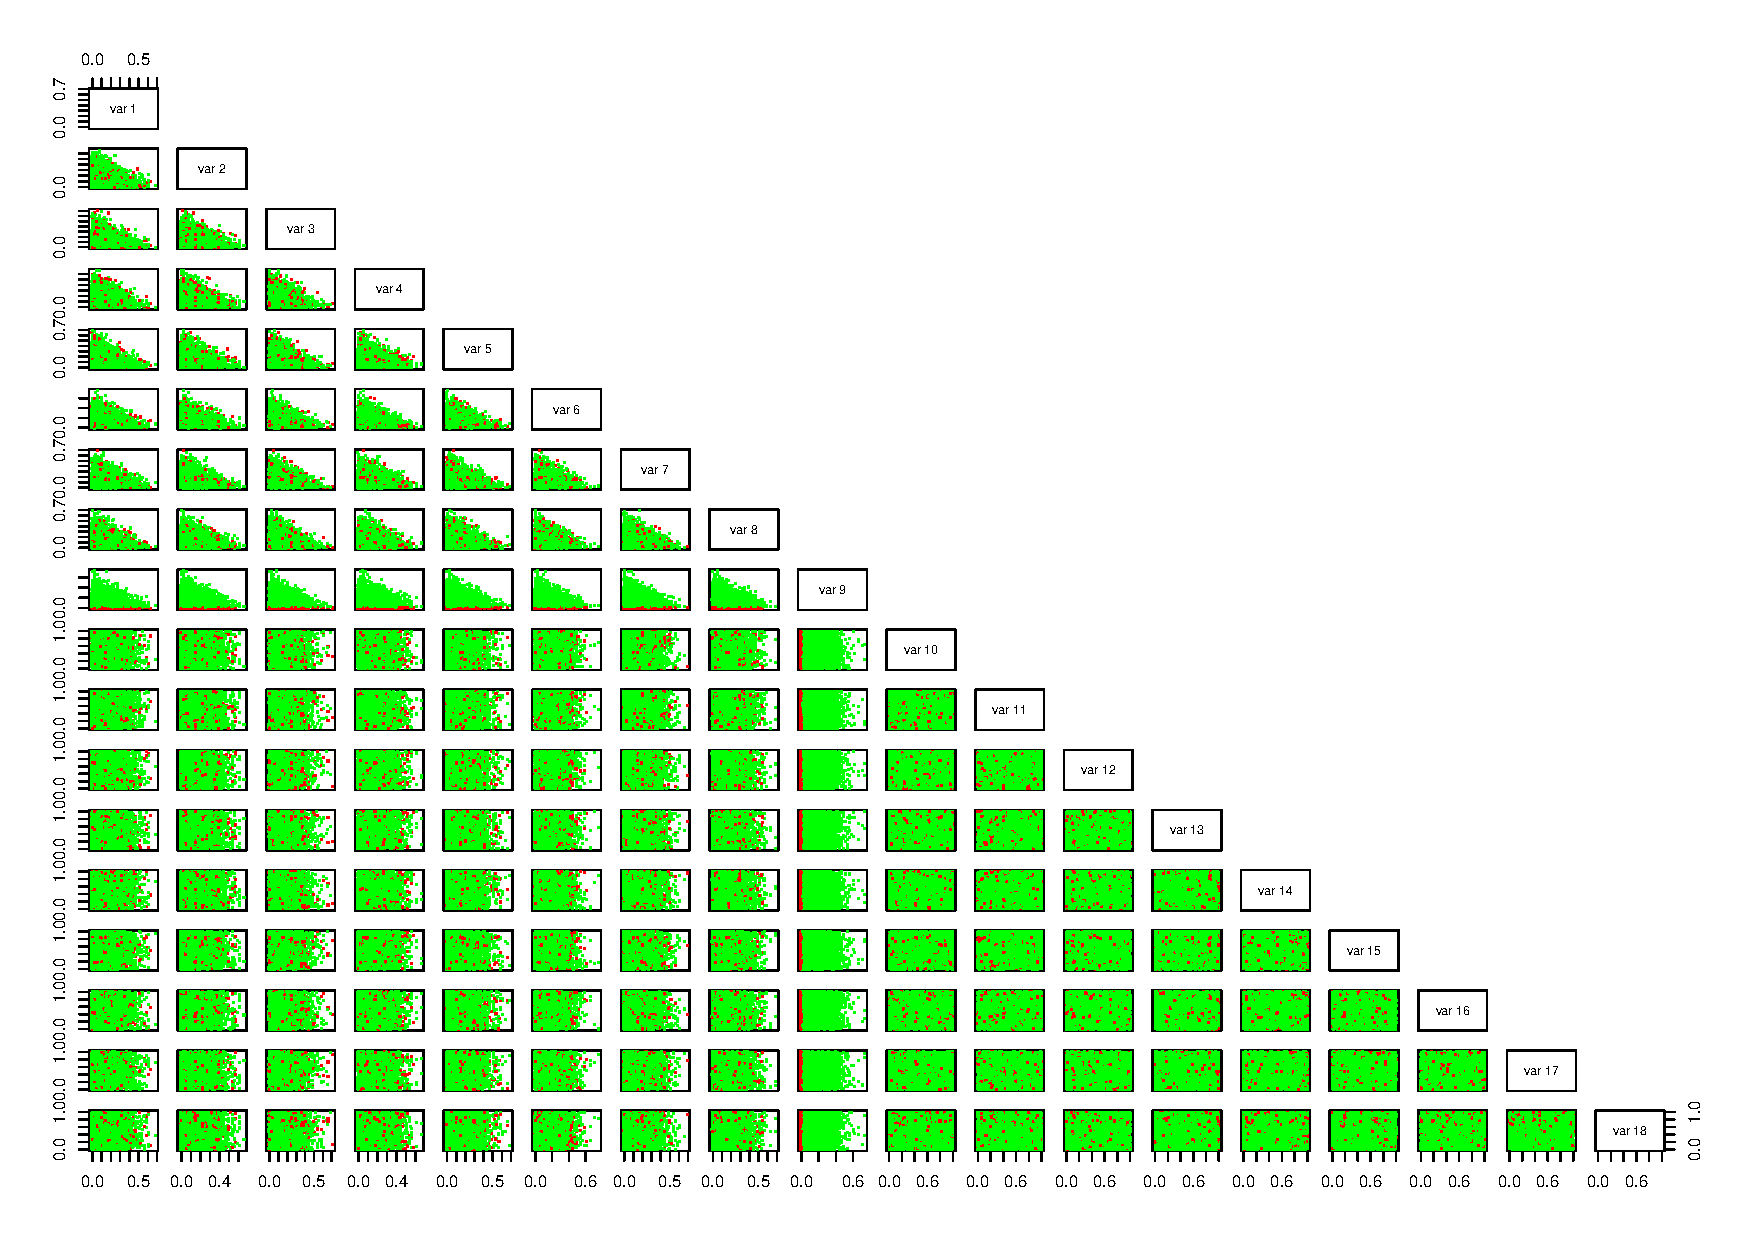
\includegraphics[width = 8in, angle=90]{fig-ds/wave1-wh1-landscape.pdf}
    \caption{A large uniform sample of decisions corresponding to Warehouse $1$. Green decisions are those that are NROY and red have been ruled out. Although $x_1$ was not included in the emulator, we have included it in this figure. Further note that the first $9$ inputs have been jittered with $\mathcal{N}(0, 9 \times 10^{-6})$ noise to aid visualisation. \label{Fig:wave1-w1-nroy}}
\end{figure}
\begin{figure}
    \centering
    \includegraphics[width = 8in, angle=90]{fig-ds/wave1-wh2-landscape.pdf}
    \caption{A collection of NROY decisions corresponding to Warehouse $2$. Although $x_1$ was not included in the emulator, we have included it in this figure.\label{Fig:wave1-w2-nroy}}
\end{figure}

We have now greatly simplified the analysis for the decision maker by applying a `post-hoc'

\subsection{Constructing a Wave $2$ Design}

We now wish to further refine the set of decisions. To do so, we need a design for a wave $2$ emulator. For Warehouse $1$, since the remaining NROY volume is quite large, simple rejection sampling will lead to a uniform design without much trouble. For Warehouse $2$, the NROY volume is a small fraction of the original volume thus rejection sampling is inefficient.

To overcome the inefficiency of rejection sampling, we employ an adapted version of the slice sampler presented by \citet{Andrianakis2017a}. The adaptation addresses the discrete simplex aspect of the decision space and is outlined in \cref{Alg:disc-slice}. The sum to unity constraint on the simplex means one decision variable is determined, given the rest. This algorithm does not include any continuous-valued components of $\bx$, however, since the algorithm is component-wise, we can first update the set of discrete components and then update the set of continuous components. We update each set in a component-wise manner.

\begin{algorithm}[h]
\caption{A single iteration of a component-wise slice sampler on the lex. \label{Alg:disc-slice}}
\begin{algorithmic}
\Require An indicator function $\mathbb{I}(\bx \in \calX_{k+1})$ for identifying inputs which are NROY, an initial NROY point $\bx_0 \in \calX_{k+1}$ where $\bx_0$ is an $m$ dimensional parameter vector. A set of $q+1$ unique, equally spaced, values $\mathcal{S} = \{ d_0, d_1, d_2, \ldots, d_{q-1},  d_q \}$ where $0 = d_0 <  d_1 < \ldots < d_{q-1}  <  d_q = 1$.
\State $\bx^{*} \gets \bx_0$
\For{$i = 1$, $2$, $\ldots$, $m$}
  \State $I^{*} \gets 0$ \Comment{Initialise an indicator variable}
  \While{$I^* \neq 1$}
    \State Compute $d_k = 1 - \sum_{j \neq i} x^{*}_j$
    \State Draw $x_i \sim \mathcal{U} \{ d_0, d_1, d_2, \ldots, d_k  \}$ \Comment{Change the $i$th input}
    \State $x^{*}_i \gets x_i$
    \State $x^{*}_1 \gets 1 - \sum_{j = 2}^m  x_j^{*}$ \Comment{Force sum to unity constraint}
    \State $I^{*}  \gets \mathbb{I}(\bx^{*} \in \calX_{k+1})$ \Comment{Evaluate the implausibility measure at the new input}
  \EndWhile
\EndFor
\State $\bx_1 \gets \bx^{*}$ \Comment{Update the $i$th component of $\bx_0$}
\State Return $\bx_1$, the new NROY sample.
\end{algorithmic}
\end{algorithm}
For low-dimensional (fewer than about 5 dimensions), continuous-valued simplices, uniform sampling gives good coverage of the margins. However, as the dimension increases, we stumble across a problem. It becomes increasingly difficult for large values of $x_i$ to be sampled.

A uniform sample on the $k$ dimensional, continuous simplex is equivalent to sampling from a $Dirichlet(1_{k+1})$ distribution, where $1_{k+1}$ is a length $(k+1)$ vector of $1$s. A well known result states that if $X \sim Dirichlet(\bm{\alpha})$ distribution are $X_i \sim Beta(\alpha_i, \alpha_0 -  \alpha_i)$ where $\alpha_0 = \sum_{j=1}^{k+1} \alpha_j$. Applying this result to the simplex means that a uniform sample on the $k$ dimensionsal simplex has $Beta(1, k)$ margins. Now for any $b \in (0,1)$, $\Pr (X_i > b) \to 0$ as $k \to \infty$. Although we have stated an asymptotic result, the effects are present even for moderate values of $k$. In \cref{Fig:beta-plot} we see plots of $\Pr (X_i > b)$ for various choices of $b$ over the range $k = lower, \ldots, 20$. Note that we have $k  = 8$ and thus $\Pr(X_i > 0.2) = $, $\Pr(X_i > 0.4) = $, $\Pr(X_i > 0.6) = $ and $\Pr(X_i > 0.8) = $. With emulators, we typically use quite small samples sizes. Typically, designs have at most $1000$ points, occasionally more are used but this is not very common. From a decision support perspeictive, this is worrying. We want to construct a design which fills the space or, at least, targets areas of the decision space which are uncertain.
\begin{figure}
  \centering
  \includegraphics{fig-ds/beta-plot.pdf}
  \caption{Lines showing how $\Pr(X_i > b)$ decreases with $k$, the dimesion of the simplex. The verticle, red dashed line corresponds to $k = 8$, the dimesion of the simplex in our wind farm example. The black lines of various types correspond to different values of $b$. Note that the verticle axis in on the logarithmic scale. \label{Fig:beta-plot}}
\end{figure}
One way to alleviate this problem is to force the design points to be far apart. This is a standard procedure. For example, maximin LHs achieve this goal by forcing the closest points to be as far away as possible. Our approach to `filling the space' will be to construct an approximate ALM design fo size $n$. This exploits the fact that GP covariance matrices depend on the design points and \textit{not} the response $y = f(\bx)$. For a single warehouse, in the following way: first construct a large, uniform design within the NROY space of sinxe $N>>n$. Call this sample $\tilde{\calX}$. Next, using assumed GP hyperparameters (from the previous wave, perhaps), find the point $\bx^{(1)} \in \tilde{\calX}$ which maximises $\var\{ U(\bx) \}$. If a constant mean function is used, all point will have equal variance thus a random sample from $\tilde{\calX}$ can initialise the procedure. We then remove $\bx^{(1)}$ from $\tilde{\calX}$ and find the next point with largest variance. Keep repeating this procedure until we have obtained $\bx^{(n)}$. Then the set $X = \{\bx^{(1)}, \bx^{(2)}, \ldots, \bx^{(n)}\}$ will be an approximate ALM design. Increaasing $N$ will likely lead to a better approximation to an exact ALM design. Finding $\argmax_{\bx \in \tilde{\calX}} \var \{ U(\bx) \}$ is achieved by computing $\var \{ U(\bx) \}$ for all $\bx \in \tilde{\calX}$. This approach is useful in two ways. Firstly is allows us to construct a space-filling design but it also allows us to perform post-processing of slice sampler. Since the slice sampler is an MCMC method, the design is prone to auto-correlation.  This post processing via ALM allows us to cope with a potentially autocorrelated MCMC chain. Rather than thinning the chain by a fixed factor (keeping every $t$-th iteraction), we automatically choose points which are not close to each other.

We used this approach for both the remaining warehouses. The slice sampler was used to generate a $N = 10^5$ candidate points for ALM designs of $n = 10^3$. For the ALM design, we utilised our knowlegde of $U(\bx)$ and used the GP hyperparameters of the emulator with mean function $h(\bx) = \beta_0 + \beta_1 \log (x_9 + 10^{-8})$. Since the emulator was fit by an empirical Bayes approach, the posterior distribution of each $(\beta_0, \beta_1)$ pair is a direct consequence of the multivariate Normal equations. Therefore, we use the wave $1$ posterior for the $\beta$ parameters as the prior for the wave $2$ emulators. This means that our ALM acquisition function, for warehouse $i$, is
\begin{eqnarray}
  \alpha_i(\bx) = K_i(\calX, X) \left\{K_i(X, X) + \lambda_i^2\right\}^{-1} K_i(X, \calX)
\end{eqnarray}
where $i \in \{1, 2\}$ denotes the choice of warehouse, $K_i(\bx, \bx') = h(\bx) B_i h(\bx)^T + C_i(\bx, \bx')$ is the GP covariance function for warehouse $i$ where $B_i = \var\{\beta^{(i)} \mid \mathcal{D}^{(i)} \}$ and $C_i(\bx, \bx')$ is covariance function for the residuals from the mean function of warehouse $i$; we assume a squared exponential covariance function. The ALM post-processing of each MCMC chain took approximately $4.5$ hours. This lead to designs which leads to $x_i$, for $i \in {1, 2, \ldots, 9}$ having wider margins than a random, uniform design of the same size. For this particular problem, our ALM approach lead to margins which, on average, were $20\%$ wider than a uniform design. This design has some interesting features. Inputs $x_{10}$--$x_{18}$ have U-shaped marginal densities. This is to be expected; uncertainty is typically largest at the edges of input spaces thus more points are places here to reduce uncertainty. We also see that for inputs $x_1$--$x_9$, the ALM design has a larger number of points close to $0$. This is because it also has more points close to $1$ and the sum to unity contraint means if $x_i$ is close to $1$, the remaining inputs must be close to $0$. This is allowing us to explore the decisions which corresponding to storing a large number of components of type $i$ which would be useful if this component was either difficult to obtain or failed much more often than other components. The uniform design would struggle to return these `extreme' decisions.

The differences between the ALM and uniform designs for Warehouse $2$ are more subtle. \cref{Fig:alm-vs-unif2} shows that, again, the range of the ALM design is typically wider than the uniform design (on average, about $10\%$ wider). Some of the uniform margins are wider then the corresponding ALM margins, but those that are wider are only wider by a small amounnt. In both cases, the difference betweent the ALM and uniform design for $x_9$ is very different. This is because we used a non-constant mean function which depends on $x_9$. If the mean function is an approapriate representation of the simulator,  this should enhance the decision support strategy. If it is not, it may hinder us. The previous diagnostic plots showed that our mean function is appropriate thus we choose to utilise our knowlegde of $U(\bx)$ to construct the designs for wave $2$.
\begin{figure}
  \centering
  \includegraphics[width = 7.5in, angle = 90]{fig-ds/alm-vs-unif.pdf}
  \caption{Comparing the marginal behvaviour of the ALM and the uniform designs for a sample size $n = 1000$ for Warehouse $1$. The ALM  design is given as the blue historgrams, whereas uniform are red. The limits of the ALM  design are the solid blue lines, the dashed red lines are the limits of the uniform design.\label{Fig:alm-vs-unif}}
\end{figure}
\begin{figure}
  \centering
  \includegraphics[width = 7.5in, angle = 90]{fig-ds/alm-vs-unif2.pdf}
  \caption{Comparing the marginal behvaviour of the ALM and the uniform designs for a sample size $n = 1000$ for Warehouse $2$. The ALM  design is given as the blue historgrams, whereas uniform are red. The limits of the ALM  design are the solid blue lines, the dashed red lines are the limits of the uniform design.\label{Fig:alm-vs-unif2}}
\end{figure}
\subsection{Wave $2$ Emulators}

To construct the wave $2$ emulators we used the ALM designs discussed above. As with the wave $1$ emulators the training data is generated by averaging over $30$ realisations of $u(\bx)$ for each $\bx$.

For the GP hyperparameters, we adopted the same priors as the wave $1$ emulators as these are realtively weak priors but chosen to omit unrealistic values of the hyperparameters. We adopted the prior mean function $\mu(\bx) = \beta^{(i)}_0 + \beta^{(i)}_1 \log (x_9 + 10^{-8})$. The prior for the $\beta^{(i)}$ was chosen as $\beta^{(i)} \sim \pi(\beta \mid \mathcal{D}_i, \Theta_i)$. That is, the posterior distributions from wave $1$ are adopted as wave $2$ prior distributions.
\begin{figure}
  \centering
  \includegraphics{fig-ds/diagnostics-wave2.pdf}
  \caption{Global diagnostics for the wave $2$ emulators. The left hand plots are for warehouse $1$ and the right hand for for warehouse $2$. The top plots show histograms of LOO errors and the bottom plots are Normal QQ plots for the LOO errors.\label{Fig:w2-global-diag}}
\end{figure}
The emulators were fit by our usual approach of assuming a Normal likelihood, integrating out $\beta$ parameters and then finding a MAP estimate of the GP covariance structure. Global diagnostics are given in \cref{Fig:wq-global-diag}. We see there is some deviation from the Normallity assumption. Namely, the left hand tail appears to be longer than the right hand tail. The excessive number of negative residuals means we would expect, on average, for the emulator's mean predictions to be slight over-predictions from the true values of $U(\bx)$. When considering the problem of optimisation under uncertainty, we would argue this is preferable to the opposite scenario of systematically under-predicting since systematic under-prediction would lead to the NROY space being smaller than it should be. However, the mean SLPE for warehouse $1$ is $-0.0452$ and the mean SLPE for warehouse $2$ is $0.00757$ which suggests that the SLPEs are not biased away from $0$. Moreover, we see that the observed proportions of SLPEs within $\pm2$ and $\pm3$ are close to their theoretical proportions, assuming Normallity (\cref{Tab:cred2}).  The observed proportions are slightly under the theoretical proportions, however, there is agreement with Pukelsheim's $3\sigma$ rule thus we are in a position to perform another round of iterative refocussing with confidence in the calibration of the approach.
\begin{table}
  \centering
  \begin{tabular}{rrrr}
    \toprule
    Warehouse & SLPE Interval & Expected Proportion & Observed Proportion \\\cmidrule{1-4}
    $1$ & $(-2,2)$&$0.95$ & $0.949$\\
    &$(-3,3)$& $0.997$ &  $0.992$ \\\cmidrule{1-4}
    $2$ & $(-2,2)$&$0.95$ & $0.946$\\
    &$(-3,3)$& $0.997$ &  $0.989$ \\\bottomrule
  \end{tabular}
  \caption{A table comparing the expected proportion to observed proportion of SLPEs to lie within given, assuming Normallity of the SLPEs for the wave $2$ emulators.}
  \label{Tab:cred2}
\end{table}
\subsection{What is the maximiser?}
Although our philosophy towards decision making views the problem as having a set of sensible solutions, rather than one optimal solution, the HM inspired approach still needs a `best' value to rule out decisions. After the first wave, taking the largest expected utility is a natural choice for `best'. However, we now have a new perspective of $U(\bx)$ provided by the wave $2$ emulator. The purpose of the wave $2$ emulator was to explore a diverse set of decisions (via an ALM design) rather than to exploit knowlegde of $U(\bx)$ to optimise it. Since the wave $2$ emulator was not designed to optimise $U(\bx)$, should we trust its maximiser?

If we plug $\hat{\bx}$ into the wave $2$ emulator, we obtain $U(\hat{\bx})  \sim \mathcal{N}(0.804, 5.63\times10^{-4})$ which is rather different to the wave $1$ prediction. This is troublesome as it is not clear how to define our implausibility measure which is reliant on the distribution of $U(\bx)$ and how it is correlated with $U(\bx')$. However, $|(0.804 - 0.831)/\sqrt(5.63\times10^{-4} + 8.75\times 10^{-5} )| = 1.08 < 3$ so these two characterisations of uncertainty about $U(\hat{\bx})$ are in some sense compatible with each other. If we search the wave $2$ design, the largest expected utility belongs to warehouse $1$ and is characterised by
\begin{equation}
  U(\hat{\bx}_2)  \sim \mathcal{N}(0.818, 2.59 \times 10^{-4}).
\end{equation}
The mean of this distribution is even closer to $\E\{U(\hat{\bx}_1)\}$
One solution to this problem is to perform a kind of sensitivity analysis: perform the analysis for both potential maximisers and see how critical the results are. To perform the sensitivity analysis we will use $\hat{\bx}_1$ and take our uncertainty about $\hat{\bx}_1$ as characterised by the wave $1$ emulator. Our uncertainty about $\hat{\bx}_2$ will be characterised by the wave $2$ emulator.

This means there will be two possible implausibility measures. They are, for $\bx \in \calX_2$
\begin{align}
  I_{2,1}(\bx) &= \frac{\E^{(1)}\{U(\hat{\bx}_1)\} - \E^{(2)} \{U(\bx)\} }{\sqrt{\var^{(1)} \{U(\hat{\bx)} \} + \var^{(2)}\{U(\bx)\}  }}\\
  I_{2,2}(\bx) &= \frac{\E^{(2)}\{U(\hat{\bx}_2)\} - \E^{(2)} \{U(\bx)\} }{\sqrt{\var^{(2)} \{U(\hat{\bx)} - U(\bx)\}  }}
\end{align}
where the $(j)$ superscript denotes the expectation/variance at the $j$th wave of emulation.  The $i,j$ subscript denotes that this is the implausibility at wave $i$ and we are using $\hat{\bx}_j$ as the `reference' value for HM.

\subsection{Second round of refocussing}
\begin{table}
	\centering
	\begin{tabular}{llrr}
		\toprule
    Wave & Best value & \multicolumn{2}{c}{Warehouse} \\\cmidrule{1-4}
    Wave $2$ only& & $1$  & $2$ \\
    &$\hat{\bx}_1$ & $88\%$ & $78.2\%$ \\
    &$\hat{\bx}_2$ & $99\%$ & $100\%$\\\cmidrule{1-4}
    Both waves& & $1$  & $2$ \\
    &$\hat{\bx}_1$ & $79.87\%$ & $1.09\times10^{-3}\%$ \\
    &$\hat{\bx}_2$ & $89.96\%$ & $1.4\times10^{-3}\%$ \\\bottomrule
	\end{tabular}
	\caption{Estimated proportion of the decision space remaining for each warehouse. The top half of the table is the reduction solely due to the wave $2$ emulators; the bottom half is the combined reduction in NROY space from both waves of emulation. \label{Tab:compare-nroy}}
\end{table}
To assess the reduction in the NROY space we first $I_{2,1}(\bx)$ as an implausibility measure. We will then use $I_{2,2}(\bx)$. Both measures will use the cut off f  $3$ to determine which points have been ruled out. To estimate the reduction in the NROY space (compared to the previous wave) we will use a random, uniform sample of $1000$ points which were deemed not implausible after the first wave of emulation. The reduction in NROY space for each warehouse, using the different implausibility measures in given in  \cref{Tab:compare-nroy}.  We see that using $\hat{\bx}_2$ as the maximiser leaves the NROY space essentially unchanged; it offers no reduction whatsoever in the space of warehouse $2$ and only removes $1\%$ of the space for warehouse $1$. Also, when treating $\hat{\bx}_2$ as the maximiser we found that $1$ of our random points lead to $I_{2,1}(\bx) < 0$. This indicates some aspects of the input space may offer a better solution than $\hat{\bx}_2$.

When using $\hat{\bx}_1$ as the maximiser, we obtain a modest reduction in NROY space for warehouse $1$ but again no reduction in the space for warehouse $2$.
\subsection{Termination of iterative refocussing}

After performing these two waves of analysis, we have used, approximately, a total of $22 \text{cores} \times 5 \text{runs} 6 \text{days} \approx 1.8 \text{years}$ of CPU time on generating training data for the emulators. This is based on the assumption that running Athena at $1000$ inputs, each replicated $30$ times will take $6$ days (over $22$ cores). Our typical training runs of Athena for this analysis all took in the region of $5$-$7$ days thus this assumption is reasonable for a back-of-the-envolope calculation. There is also the issue of queueing on HPC facilities which can be of the order of several days during busy periods. In terms of wall-clock time, we used a total of around $14$ days computing time (different jobs started and ended at different times). Another round of emulation would take approximately another $6$ days in training time. None of our calculations have included the human time or additional computational cost of fitting or validation of emulators or the computational cost of a design. For this reason, combined with the modest reductions in NROY space we now terminate out iterative procedure as we belive further computations would not provide a worthwhile reduction in the NROY space.

\section{Incorporating the DM: Evaluating the consequences of decisions}

In final aspect of our analysis contains two parts. First we will provide the decision makers with a small set of decisions from the NROY space. These are decisions which are not clearly worse than $\hat{\bx}_1$. We will present the decision to the DM alongside the consequences if that decision. Note that the consequences are the choice of warehouse, the availablity time series and the restoration policy. We will present multiple replicates of the availablity  times series to the decision maker to communicate that this is an uncertain consequence.

The decision maker then has two tasks. The first task is to provide feedback on the decision space. If the decision makers finds all the solutions unsatisfactory, we must go back to the start of our analysis and perform the entire task again. re-elict attributes, consequences, the functional form and parameters of the utility function. Prior to doing this however, there are some `sanity checks' that could be performed.

For example, since we only present the DM with a small sample of decisions from the NROY space, if the DM finds no decision satisfactory from the sample, it would be worthwhile considering a different sample of decisions. Note that this step is computationally expensive because one consequence relies on running the Athena simulator. However around $30$ replicates for a handful of say $5$ decisions can be computed in about an hour on the Rocket HPC facility or perhaps overnight on a desktop computer with $8$ cores. If the analyst is still not happy with the results, it may be worth trying to optimise a single consequence. For example, if the DM was not happy with the availablity trajectories we have produced from the NROY space, it would be worth investigating if there are \textit{any} availablity trajectories within the initial decision space that the DM is happy with.

If the decision makers finds one or more solutions satisfactory, they must then decide which decision to make. This decision should soley be that of the decision maker.

\subsubsection{Final NROY volume}

\section{Conclusions}

We have presented a history matching inspired procedure for decisions support with the Athena simulator. Our approach drew on established ideas but relied on novel applications of ideas to address the challenges within our wider problem of decision support for Athena.

We first provided an illustrative elicitation of a utility function. We drew on key attriutes to the problem but we stress the elicitation will always be subjective. Therefore, every decision maker will have their own utility function.

We then proposed joining together two established approaches. We began by performing three independent rounds of Bayesian optimisation then used techniques from the HM literature. Our HM inspired approach required a novel implausibility measure  which incorporated the dependence across the decision space. This was necessary as we ruled out decisions based the value of one of the other emulator runs, thus $U(\hat{\bx})$ is informative for $U(\bx)$ when $\bx$ is close to $\hat{\bx}$.

We then considered design for our decision support exercise. BayesOpt allowed us to side-step the problem of design for a wave $1$ emulator since it automatically chooses where to run the simulator. The design for a wave $2$ emulator was more challenging as we had to adhere to the constraints of the decision task a whilst  constructing a design within the NROY region that provided a diverse set of decisions. We chose another sequential design approach. Our approach also incorporated out choice of mean function to produce an `optimal' design. This design will only be optimal if our choice of mean function is also plausible. If the analysis were to be performed again, it may be worth investigating this modelling choice. To increase the flexibility of the design, the analysis could use an ALM design but assume a constant mean function for the GP. The GP hyperparameters may need to be re-estimated for this design (or simply specified) as the choice of mean function will, in general, alter the GP hyperparameters.

We then constructed a new pair of emulators to further explore the NROY space. We performed a sensitivity analysis based on the choice of possible maxima. One maximum lead to a negligible reduction in the NROY space and the other lead to a small reduction in the NROY space. In general, we would advise using the results of the BayesOpt routine to choose the maximiser. This is because that round of emulation was designed to find the largest value of $U(\bx)$ possible. If, however, a later round of emulation provides us with an improved option it would be worth using the improved option as a reference value.

Finally, we presented the DM with a set of sensible decisions that could be taken. We presented decisions from both warehouses and from diverse decisions within each warehouse. This should help to challenge the decision maker and force them to think carefully about the consequences of their decision. We stressed that if the DM is not happy with the consequences of NROY decisions, that the analyst and DM should be willing to go back to the start of the analysis and carefully check the DM's utility function.

\end{chapter}
